% !TEX root = main.tex

\section{Overview}

Symbolic execution has been originally introduced in~\cite{K-ACM76} and~\cite{H-TSE77}. A good introduction to symbolic execution is present in~\cite{KLEE-OSDI08} (while~\cite{EXE-CCS06} is a previous effort of the same authors). \cite{SAGE-NDSS08} is one successful story of symbolic execution. \cite{SAB-SP10} presents a neat formalization of symbolic execution (and taint analysis).

\subsection{Motivation}

Symbolic execution is a static analysis technique that have been introduced to perform automatic testing of complex software. For instance, consider the C function shown in Figure~\ref{fig:example-1}. A critical operation performed by this code is the division performed on line 10. Testing techniques such as random testing can generated several input tests for this function. However, it is unlikely that the inputs which make this code crash are effectively picked up by these techniques. Indeed, although this code is relatively simple, there are too many possible assignments to the input values {\tt a}, {\tt b}, and {\tt c}. In general, each {\tt int} input variable in C has $2^{32}$ possible values. In practice, only input values which lead to $x + y + z - 3$ equal to zero make the code crash.

Symbolic execution overcomes common limitations of random testing techniques by evaluating a piece of code using {\em symbols}, instead of concrete values for the inputs. The main idea is to consider classes of input values, instead of a single instance values. Before analyzing how symbolic execution can identify the proper inputs which will make the function {\tt foobar} crash, we need to introduce few basic definitions.

\subsection{A simple execution model}
\label{simple-execution-model}

Symbolic execution is a methodology for executing a program symbolically. At any point of the execution, a state is kept by the symbolic execution engine.

\paragraph{Symbol} Any local or global variable is associated to a symbol $\alpha_i$. 
\paragraph{Execution state} The execution state $(stmt,~pc)$ is composed by two kinds of information:
\begin{itemize}
  \item $stmt$: the next statement that should be evaluated
  \item $pc$: path constraints, i.e., set of assumptions made over the symbols $\alpha_i$ to reach the statement $stmt$. Initially the $pc$ is empty, i.e., set to true.
\end{itemize}
Since, in general, any memory location may have associated a symbol, it is common to maintain a memory mapping $M$ for storing constraints associated to different symbols.

\paragraph{Execution model} Depending on the kind of the statement $stmt$, the execution state is modified as follows:
\begin{itemize}
  \item (constant assignment) $\alpha_i = c$: when a constant value $c$ is assigned to a variable associated to the symbol $\alpha_i$, $pc$ is extended, adding the constraint:
    \[ pc \gets pc \wedge \alpha_i = c\]
  \item (assignment) $\alpha_i = e$: when an expression $e$ is assigned to a symbol $\alpha_i$, $pc$ is extended, adding the constraint:
    \[ pc \gets pc \wedge \alpha_i = e\]
  where $e$ can be any expression, such as unary or binary operation, over symbols and constants.
  \item (conditional branch) {\tt if} $e$ {\tt then} $stmt_{true}$ {\tt else} $stmt_{false}$: $pc$ is evaluated. Two scenarios are possible:
    \begin{itemize}
      \item (non-forking) $e$ is always verified (true) or always not verified (false): the proper branch is taken, evaluating $stmt_{true}$ or $stmt_{false}$.
      \item (forking) the boolean value of $e$ is not determinable without instantiating the values of one or more symbols: the symbolic execution is forked, creating two parallel execution states:
        \[ (stmt_{true}, pc_{true}) \text{ where } pc_{true} = pc \wedge e \]
        \[ (stmt_{false}, pc_{false}) \text{ where } pc_{flase} = pc \wedge \neg e \]
    \end{itemize}
    The execution is proceeded on both states.
  \item (jump) {\tt goto} $stmt$: the execution state is updated to match the given next statement to be evaluated. 
  \item (other constructs) A discussion of other constructs such as $call$, $return$, $while$, or $for$ is provided in Section~\ref{example-discussion}. 
\end{itemize}

\subsection{Example}
\label{symbolic-execution-example}

\begin{figure}[t]
\begin{lstlisting}[basicstyle=\ttfamily\small]
              1.  int foobar(int a, int b, int c) {
              2.    int x = 0, y = 0, z = 0;
              3.    if (a != 0)
              4.      x = -2;
              5.    if (b < 5) {
              6.      z = 2;
              7.      if (a == 0 && c != 0)
              8.        y = 1;
              9.    }
             10.    return a / (x + y + z - 3);
             11.  }
\end{lstlisting}
\label{fig:example-1}
\caption{Example: a very simple C function}
\end{figure}

\begin{figure}[t]
  \centering
  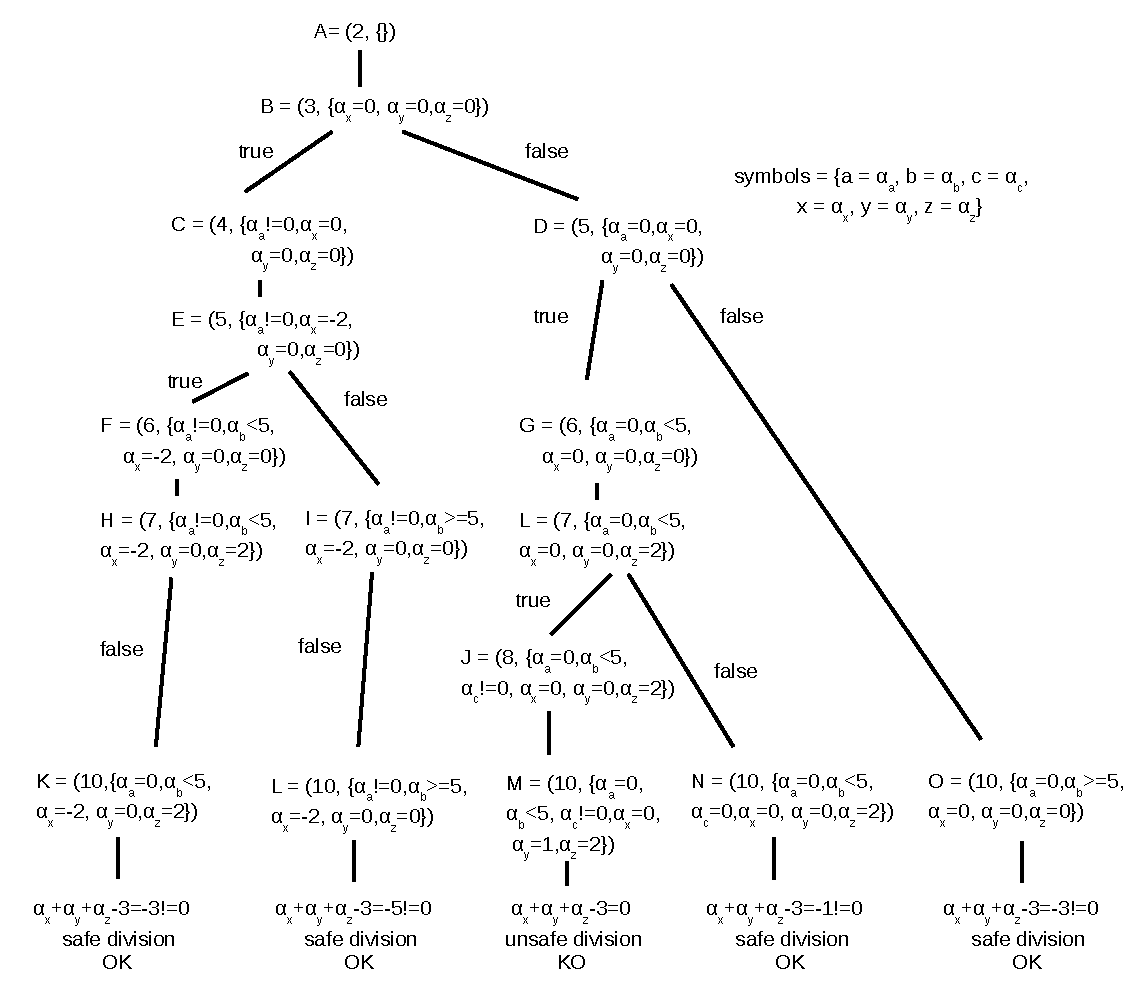
\includegraphics[width=1.0\columnwidth]{images/example} 
  \caption{Symbolic execution tree of the function {\tt foobar}. Each execution state is labeled with an alphabet letter. Side effects on execution states are highlighted in gray. Leaves are evaluated against division by zero error. For the sake of presentation the conjunction of constraints is shown as a list of constraints. }
  \label{fig:example-symbolic-execution}
\end{figure}

The symbolic execution of the function {\tt foobar} is shown in Figure~\ref{fig:example-symbolic-execution}. Initially, a new symbol is introduced for each input argument and for each local variable. For the sake of the presentation, we have associated symbol $\alpha_{var}$ to the variable $var$. Moreover, we have assumed to know the set of local variables used by the function. In general, obtaining this information may be non trivial and thus it it common to introduce symbols related to local variables only when the statements defining the variables are evaluated. To track the mapping between variables and symbols, a mapping table is maintained. 

The first statement of the function is line 2. For this reason, the initial execution state $A$ is given by $(2, \{\})$ where the path constraint set is empty since no assumption can be made on any symbol. After executing line 2, the $pc$ is updated adding constraints on the value of $\alpha_x$, $\alpha_y$, and $\alpha_z$ (see execution state $B$). Line 3 contains a conditional branch: since the condition cannot be uniquely resolved based on the current set of assumptions, the execution is forked. Depending on the taken branch, a different statement is next evaluated and different assumptions are made on the symbol (see execution state $C$ and $D$). On the other hand, if the condition can be uniquely determined such as when evaluating the execution state $H$, then there is not need to fork the execution but it is sufficient to follow only the interesting branch (e.g., $L$ from $H$), pruning away unrealistic execution states. 

After expanding any execution state until it reaches the statement on line 10, we can finally check which values for the input parameters {\tt a}, {\tt b}, and {\tt c} make the function {\tt foobar} crash by performing a division by zero operation. Analyzing execution states $\{L, M, N, O, P\}$, we can conclude that only the execution state $N$ can lead to an unsafe operation. The path constraint set of $N$ defines the set of inputs which are unsafe for function {\tt foobar}. Any input parameters for $\alpha_a$, $\alpha_b$, and $\alpha_c$ such that:
 \[ \alpha_a = 0 \wedge \alpha_b < 5 \wedge \alpha_c \neq 0 \]
will crash this function. An instance of unsafe input parameters for {\tt foobar} can determined exploiting a constraint solver (i.e., an oracle able to resolve constraints). For instance, given the execution state $N$, a solver may come up with the values $a = 0$, $b = 1$, and $c = 0$. Notice that a constraint solver is also needed when evaluating the satisfiability of branch conditions. 

\subsection{Discussion}
\label{example-discussion}

The example described in Section~\ref{symbolic-execution-example} shows the effectiveness of the symbolic execution methodology in finding {\em all} the possible unsafe input values which may trigger a crash due to an unsafe division performed at line 10. This is achieved by symbolic execution through an exhaustive exploration of all the possible execution states. For this reason, at least from a theoretical point of view, symbolic execution can be seen as a sound and complete approach. This means that if an input values is detected as unsafe then it is actually unsafe. Moreover, symbolic execution is able to always find all the unsafe inputs. However, real-world code can be significantly more complex than the example shown in Figure~\ref{fig:example-1}. Several observations and questions naturally arise:

\begin{enumerate}

  \item (objects) {\em How does symbolic execution handle arrays or other more complex objects?} \\
  In general, any arbitrary complex object can be seen as an array of bytes, where each byte can have associated a distinct symbol. Indeed, even a C {\tt int} type can be seen as an array of four bytes. In practice, it is convenient, whenever possible (e.g., by statically analyzing the source code), to exploit structural properties of the data. 

  \item (loops) {\em How does symbolic execution handle loops?} \\
  Using the execution model presented in Section~\ref{simple-execution-model}, a loop can be evaluated by translated it into a combination of conditional branches and $goto$ statements. This transformation is not uncommon when a high-level language like C is compiled into binary code. However, the main critical aspect when symbolically executing a loop is choosing how many iterations should be analyzed. In general, a loop may be repeated depending on the value of some variables whose values may be not constant, e.g., the number of iterations is given by the value of an input parameter. The naive approach can lead to create a new execution state for each possible repetition of the loop.

  \item (subroutines) {\em How does symbolic execution handle subroutines?} \\
  The execution model presented in Section~\ref{simple-execution-model} does not specify how to handle invocation to subroutines (i.e., a $call$ statement). An way to extend our execution model in order to handle subroutines it to expand the execution state by adding a simple execution stack.

  \item (recursion) {\em How does symbolic execution handle recursion?} \\
  Consider, as an example, the code:
    \begin{lstlisting}[basicstyle=\ttfamily\small]
    1.  int bar(int n) {
    2.    if (n >= 0) 
    3.      return 0;
    4.    return 1 + sum(n - 1);
    5.  }
    \end{lstlisting}
  Assuming to have introduced an execution stack in the execution state, it can be easily observed that the above can easily lead to a very large number of executions states. Indeed, the number of executions states is related to the number of times that the conditional branch on line 2 is not taken. 

  Since the {\tt int} type in C can have $2^{31} - 1$ positive values, symbolic execution has to create more than $2^{31} - 1$  execution states to cover all the possible execution paths.
 
  \item (environment) {\em How does symbolic execution handle interaction with the environment}? 
  Real-world applications interacts constantly with the environment: this is typically achieved by invoking library or system routines. A crucial aspect of these interactions is that they may cause some side-effects on the environments (e.g., creation of a file or initialization of a memory area) which must be considered since they may affect the actual execution of the code. Evaluating any possible outcome of an interaction is not feasible in most scenarios due to the large number of execution states which could be required. Moreover, it is likely that only a very small subset of this outcome is actually realistic. Hence, it is common to create models for popular library and system routines that help the symbolic execution engine to consider only significant outcomes.

  \item (state space explosion, path selection) {\em How does symbolic execution deal with path explosion}? \\
  A relatively simple code such as function {\tt foobar}, which is composed by less 12 lines of code, has generated 16 execution states, where $5$ out of $16$ are independent and must be checked to determine possible unsafe input values. Although this could seem a reasonable number of states, few lines of code, such as loops, may contribute to exponentially increase the number of states. For this reason, it is unlikely that a symbolic execution engine is able to exhaustively explore all the possible execution states within a reasonable amount of time. In practice, several heuristics must be exploited to prioritize evaluation of some states, hoping to still be able to spot interesting things. Moreover, the symbolic execution engine should include efficient mechanism for efficiently evaluating in parallel different execution states without running out of computational resources.

  \item (constraint solver) {\em What is a constraint solver in practice}? \\
  Constraint solvers exist in practice but they have significant limitations. A common limitation is that they are able to solve complex constraints in a reasonable amount of time only if these constraints are composed by linear expression over the symbols $\alpha_i$. For this reason, it is common to integrate optimizations in the symbolic execution engine that are able to generate {\em solver-friendly} constraints.

  \item (binary code) {\em What are the disadvantages of symbolically executing binary code}? \\
  The example presented in Section~\ref{symbolic-execution-example} is written in C. This does not mean that symbolic execution cannot be performed directly on binary code. However, having the source code of an application can significantly make it easier its symbolic execution since several sound assumptions can be obtained by statically analyzing the source code (e.g., the maximum size of a buffer or the number of iterations for a loop).
   
\end{enumerate}
Depending on the specific application context of symbolic execution, different choices and assumptions are made to address the above questions. Although soundness and completeness of symbolic execution may be negatively affected by these choices, there are several application scenarios where a partial exploration of the possible execution states is sufficient for reaching the ultimate goal (e.g., identify a single input that crashes an application).


%%%%%%%%%%%%%%%%%%%%%%%%%%%%%%%%%%%%%%%%%%%%%%%%%%%%%
\section{Memory model}
A crucial aspect of symbolic execution is how the memory should be modeled. In other words, a symbolic engine may see symbols as distinct objects (i.e., each symbol is a distinct array of a specific size) or as pointers to a flat memory (i.e., index-based memory). Although the latter approach may seem more natural since it is akin to a concrete execution model, the former has been proved to be very effective in many scenarios since the symbolic constraints generated when using this approach are {\em easier} to parse for some solvers.

\subsection{Index-based memory~\cite{MAYHEM-SP12}}
\begin{itemize}
  \item memory is a map $\pi : I \to E$ from 32-bit indices ($i \in I$) to expressions ($e \in E$)
  \item load expressions $e = load(\pi, i)$: $i$ indixes $\pi$ and the loaded value $e$ represents the contents of the $i$-th memory cell
  \item store expressions $store(\pi, i, e)$: a new memory $\pi'$ where $i$ is mapped to $e$, i.e., $\pi' = \pi[i \gets e]$
\end{itemize}
When using this memory model, handling of arbitrary symbolic indices is notoriously hard, since a symbolic index may reference any cell in memory. Two approaches can be pursued: (a) concretization of the index where only a single value is evaluated for the index (see Section~\ref{concolic-execution} for more details), (b) fully symbolic memory where any possible value for the index is evaluated (e.g., \cite{BAP-CAV11}). The former is often excessively limiting (many paths are pruned away), while the latter is hard to make scalable. To overcome the limitations of both approaches, \cite{MAYHEM-SP12} models memory {\em partially}: symbolic writes are always concretized, while symbolic reads are allowed to be modeled symbolically.

\paragraph{Memory objects} Whenever there is a symbolic read, an immutable memory object $\mathcal{M}$ is generated:  it contains all values that could be accessed by the index, i.e., $\mathcal{M}$ is a partial snapshot of the global memory $\pi$. In practice, \cite{MAYHEM-SP12} reasons on $\mathcal{M}[i]$ instead of reasoning on $\pi[i]$, since the former is typically smaller than the latter.

\paragraph{Memory object bounds resolution} \cite{MAYHEM-SP12} trades accuracy with scalability by resolving the bounds $[\mathcal{L}, \mathcal{U}]$ of the memory region, where $\mathcal{L}$ is lower and $\mathcal{U}$ is the upper bound for the index $i$. Initially, $\mathcal{L} \in [0, 2^{32}-1]$. The solver is used to test if $i < \frac{2^{32}-1}{2}$ makes the path constrains unsatisfiable. If satisfiable then $\mathcal{L} \in [0, \frac{2^{32}-1}{2}]$, otherwise $\mathcal{L} \in [\frac{2^{32}-1}{2}, 2^{32}-1]$. The same strategy is repeated as much as possible. This is akin to a binary search algorithm. Whenever the bounds become reasonable, a memory object is generated. Unfortunately, there several cases where the bounds cannot be narrowed down drastically and thus other techniques can be used:
\begin{itemize}
  \item {\em value set analysis (VSA)}
  \item {\em refinement cache}
  \item {\em lemma cache}
  \item {\em index search trees (IST)}
  \item {\em bucketization with linear functions}
\end{itemize}
Whenever the size of the memory object exceeds a threshold (e.g., $|\mathcal{M}| \geq 1024$), then~\cite{MAYHEM-SP12} concretizes the index. However, instead of choosing a random value for the index, it tries to assign some {\em interesting} value (e.g., test it if it makes sense for it to be equal to an invalid memory address which can be exploited for security purposes).

\subsection{Object-based memory~\cite{EXE-CCS06,STP-TR07}}

\cite{STP-TR07} is a decision procedure for bitvectors and arrays. Memory is seen as untyped bytes. Three data types are available:
\begin{itemize}
  \item {\em booleans}
  \item {\em bitvectors}: a fixed-length sequence of bits
  \item {\em arrays of bitvectors}
\end{itemize}
Most linear and non-linear operations are mapped to bitvector constraints. Conditional branches are transformaed into {\em multiplexers}, which are similar to C ternary operator. Bitvector operations are translated into operations to individual bits. Floating-points data types are not supported. Expresions types:
\begin{itemize}
  \item {\em formulas}, which have boolean values. They are converted into DAGs of single bit operations, where expressions with identical structure are represented uniquely (an hash table is maintain to track of existing expressions and lookups are performed on it when a new expression is created).
  \item {\em terms}, which have bitvectors values. They are converted into vectors of boolean formulas consisting entirely of single bit operations.
\end{itemize}

\paragraph{Mapping C code to STP primitives} Each C data block is represented symbolically as an array of 8-bit bitvectors. Typed operations in C generated constraints on the symbolic data (i.e., typeness is not actually known to~\cite{STP-TR07}). A mapping table is maintained to track symbolic data:
\begin{itemize}
  \item each input array $b$ is associated to a symbolic identically-size array $b_{sym}$ (i.e., the address of the C variable $b$ is mapped to the symbolic array $b_{sym}$ that is composed by $|b|$ 8-bit elements)
  \item $v = e$: an assignment expression, where $e$ is an expression that involves one or more symbolic data, adds a mapping between the address of $v$ and the generated symbolic expression $e_{sym}$. If $v$ is overwritten with a constant value or deallocated then this mapping is removed.
  \item $b[e]$: $b_{sym}$ is allocated, initializing it with the (constant) contents of $b$ (only if $b$ is actually initialized by a previous C statement). A mapping is added until $b$ is not deallocated.
\end{itemize}

\paragraph{Expression evaluation} An expression $e$ that contains some symbolic data can be seen as:
\[ l_1~~op_1~~l_2~~op_2~~l_3~~... \]
Each $l_i$ is evaluated in the following way:
\begin{itemize}
  \item if $l_i$ is concrete: the concrete value is used in the expression (e.g., if 4-byte $b$ is equal to 4 then the constant $000000...0100$ is used)
  \item otherwise: a concatenation of all the symbolic bytes of $l_i$ is used (e.g., $b_{sym}[0] @b_{sym}[1] @ $ $b_{sym}[2] @ b_{sym}[3] @ ...$)
\end{itemize}
Pointers are seen as array reference at some offset. This means that allocation sites as well as pointer arithmetic expressions must be instrumented in order to track where a pointer can point to. Notice that double dereferences ({\tt **p}) force~\cite{STP-TR07} to concretize the first dereference ({\tt *p}). 

\paragraph{Fast array transformations} Some transformations are needed to make\cite{STP-TR07} reason only on a purely functional language. In particular:
\begin{itemize}
  \item {\em read-over-write}: eliminates all write operations
    \[ read(write(A, i, v), j) \implies ite(i = j, v, read(A, j)) \]
    where $ite(a,b,c)$ is a ternary operator (i.e., if $a$ then $b$ else $c$). Notice that a write of a location without a subsequent read of the same location can be ignored.
  \item {\em read elimination}:
    \[ (read(A, i) = e_1) \wedge (read(A, j) = e_2) \]
    will be transformed in:
    \[ (v_1 = e_1) \wedge (v_2 = e_2) \wedge (i=j \implies v_1 = v_2) \]
  \item {\em array substitution optimization}
  \item {\em array-based refinement}
  \item {\em simplifications}: boolean or mathematical identities
\end{itemize} 

\paragraph{Optimizations} Other optimizations are applied:
\begin{itemize}
  \item {\em constraint caching}: cache solver results and reuse them
  \item {\em constraint independence}: tracks constraints into multiple independent subsets of constraints, This helps the system discards irrelevant constraints and adds additional cache hits.  
\end{itemize}

\section{Loops}

A technique to make it easier to perform symbolic execution on loops is through imposing some preconditions. See Section~\ref{precontioned-symbolic-execution} for more details.

\section{Interaction with environment}

Environment can be seen as an input source. Since it can be unfeasible to analyze all possible interactions with the environment, it is common to model these interactions, emulating their behaviors and their side-effects. The main intuition is that models understand the semantics of the desired actions well enough to generate the required constraints.\\

\cite{KLEE-OSDI08}:
\begin{itemize}
  \item {\em file system}: operations on concrete files are actually performed. Operations on symbolic files are emulated modeling a simple symbolic file system, which is private for each execution state. Symbolic file system is a directory with $N$ symbolic files. Users specify both the number of files and their sizes. Any operation on a unconstrained symbolic file will generate $N+1$ branches: one for each symbolic file, plus one for a failing scenario. Emulation done at library level, not system call level. This make symbolic execution simpler (no need to symbolically execute library code) but assumption that library code is correct. If needed, library code is tested separately.
  \item {\em environment failures}: \cite{KLEE-OSDI08} emulates failures (e.g., failures of {\tt write}). This is optional since some applications may be not sensitive to environment failure.
  \item {\em re-running test cases}: inputs which may crash an application may depend on the environment failures. To force concrete execution towards failures, \cite{KLEE-OSDI08} exploits {\tt ptrace}.
\end{itemize}

\cite{AEG-NDSS11}:
\begin{itemize}
  \item {\em symbolic files}: emulation of {\tt open}, {\tt read}, {\tt write}, and similar other system calls. Similar to~\cite{KLEE-OSDI08}.
  \item {\em symbolic sockets}: emulation of {\tt socket}, {\tt bind}, {\tt accept}, {\tt send}, and similar other system calls. 
  \item {\em environment variables}: a complete summary of all possible results (concrete values, fully symbolic, and failures) of {\tt get\_env}.
  \item {\em library function calls and system calls}: emulation of more than 70 library routines and system calls. In particular, formatting functions (e.g., {\tt fprintf}) are emulated to capture buffer overflows.
\end{itemize}

\cite{DART-PLDI05}: external interfaces are extracted by analyzing library and system calls, then random results are returned (compliant with the type).

\section{State space explosion}

\subsection{Preconditioned symbolic execution~\cite{AEG-NDSS11}}
\label{precontioned-symbolic-execution}

The main challenge with symbolic execution is managing the state space explosion problem. Since symbolic execution forks off a new interpreter at every (undecidable) branch, the total number of interpreters is exponentially in the number of of branches.\\

\cite{AEG-NDSS11} have proposed {\em preconditional symbolic execution} as a novel method to target symbolic execution towards certain subset of the input state space. The state space subset is determined by the precondition predicate $\Pi_{prec}$: inputs that do not satisfy $\Pi_{prec}$ will not be explored. The intuition for preconditioned symbolic execution is that we can narrow down the state space we are exploring by specifying exploitability conditions as a precondition, e.g., all symbolic inputs should have the maximum size to trigger buffer overflow bugs. The main benefit from preconditioned symbolic execution is simple: by limiting the size of the input state space before symbolic execution begins, we can prune program paths and therefore explore the target program more efficiently.
Note that preconditions cannot be selected at random. If a precondition is too specific, we will detect no bugs or exploits; if it is too general, we will have to explore almost the entire state space. %Thus, preconditions have to describe common characteristics among exploits (to capture as many as possible) and at the same time it should eliminate a significant portion of non-exploitable inputs.\\

Preconditioned symbolic execution enforces the precondition by adding the precondition constraints to the path predicate during initialization. Adding constraints may seem strange since there are more checks to perform at branch points during symbolic execution. However, the shrinking of the state space -- imposed by the precondition constraints -- outweighs the decision procedure overhead at branching points. When the precondition for a branch is unsatisfiable, we do no further checks and do not fork off an interpreter at all for the branch.% We note that while we focus only on exploitable paths, the overall technique is more generally applicable.\\

\paragraph{Preconditions} Kinds of preconditions:
\begin{itemize}
  \item {\em None}. There is no precondition and the state space is explored as normal.
  \item {\em Known Length}. The precondition is that inputs are of known maximum length. Static analysis techniques can be used to automatically determine this precondition.
  \item {\em Known Prefix}. The precondition is that the symbolic inputs have a known prefix.
  \item {\em Concolic Execution}. Concolic execution [24] can be viewed as a specific form of preconditioned symbolic execution where the precondition is specified by a single program path as realized by an example input. For example, we may already have an input that crashes the program, and we use it as a precondition to determine if the executed path is exploitable. See Section~\ref{concolic-execution} for a more detailed discussion of this technique.
\end{itemize}

\paragraph{An example} Consider the example:

\begin{lstlisting}[basicstyle=\ttfamily\small]
    // N symbolic branches 
    if (input[0] < 42) [...]
    [...]
    if (input[N - 1] < 42) [...]

    // symbolic loop
    strcpy(dest, input); 

    // M symbolic branches
    if (input[N + 1] < 42) [...]
    [...]
    if (input[N + M - 1] < 42) [...]
    \end{lstlisting}
where {\tt input} is an array of {\tt S} bytes. Impact of preconditions:
\begin{itemize}
  \item {\em None}. No constraint is added. State space is $2^N \cdot S \cdot 2^M$.
  \item {\em Known Length}. For instance, we add constraint that $(S - 1)$ bytes of {\tt input} are not equal to \textbackslash0. Since the symbolic loop is known, then the state space is reduce to $2^N \cdot 2^M$.
  \item {\em Known Prefix}. For instance, we add constraint that the $P$ bytes of {\tt input} are known ($P < N < S$). E.g., fixed header string). Since first $P$ branches and first $P$ iterations are concrete, then state space is $S \cdot 2^{N-P} \cdot 2^M$.
  \item {\em Concolic Execution}. We decide the exact values for all bytes of {\tt input}. Input space is $1$.
\end{itemize}

\subsection{Concolic execution}
\label{concolic-execution}

{\em Concolic execution} has been originally introduced in~\cite{DART-PLDI05} and then refined by~\cite{CUTE-FSE13}. A common disadvantage of symbolic execution is that the state space can be exponential. Moreover, even when the state space is tractable it may happen that complex constraints need to be solved but these constraints are too complex for the actual solver (e.g., non-linear constraints are typically hard to solve). For this reason, it is common to exploit concolic execution. Different scenarios:
\begin{itemize}
  \item {\em Use concolic execution to generate useful random inputs.} Starts concrete execution using a random (concrete) input and for each taken branch tracks the input constraints by observing the branch condition. When the execution is completed, restart another concrete execution using a different concrete random input that is compliant with the constraints but explore a new path. It is sufficient to negate a single constraint given by a conditional branch, to explore a different path. Keep track of taken branches with binary values. An algorithm for maximizing coverage is proposed in~\cite{DART-PLDI05}. Notice that the symbolic execution is performed in parallel with the concrete execution.
  \item {\em Use concolic execution to overcome unsolvable constraints}. Assume to start a concrete execution with a concrete input and in parallel symbolically execute the same program. Whenever a set of constraints cannot be solved by the constraint solver, then use the concrete value to proceed into at least one branch. Use concrete values also to avoid to perform alias analysis on pointers, which is typically very expensive. Whenever meaningful, \cite{DART-PLDI05} tries to test both valid (not {\tt NULL}) and invalid ({\tt NULL}) input pointers in order to maximize bug detection. However~\cite{DART-PLDI05} will never artificially negate a branch if that condition cannot be exercised using a concrete input. In other words, both branches of an {\tt if} statement are considered only if they are both meaningful (more precisely: \cite{DART-PLDI05} is able to generate a valid input). Notice that~\cite{DART-PLDI05} may generate an input using a solver by considering only a subset of branch constraints. For instance, consider constraints ($C_1, C_2, C_3$) given by three nested branches: if $C_1$ is non linear (hard to solve), it needs only to generate a random input for taking $C_1$ and then use the solver for exploring path given by $(C_2, C_3)$. A traditional symbolic execution engine may get stuck at $C_1$ and give up after some time on {\em all} the derived path. Notice that whenever a concrete input is used to overcome a hard constraint, the overall approach become incomplete.
\end{itemize} 

\section{Symbolic executors}
A symbolic execution engine should guarantee three main principles (\cite{MAYHEM-SP12}):
\begin{enumerate}
  \item the system should be able to forward progress for arbitrarily long time, ideally forever, without exceeding the given resources
  \item to maximize performance, no work should be repeated (avoid to restart symbolic / concrete execution)
  \item the system should reuse as much as possible previous analysis results
\end{enumerate}

Based on these principles, symbolic executors can be divided into:
\begin{itemize}
  \item {\em offline} executors (e.g., \cite{SAGE-NDSS08}): one path at time, every run independent from the others, results can be immediately reused, each run restarts the execution of the program from the beginning. In order to perform a run, two inputs must be provided: the target program and a seed input. The program is concretely executed and a trace is recorded. Then the trace is symbolically executed. This can be seen as a form of {\em concolic} execution (see Section~\ref{concolic-execution}).
  \item {\em online} executors (e.g., \cite{KLEE-OSDI08,CKC-TOCS12,AEG-NDSS11}: for each fork, the execution state is cloned. All active execution states are kept in memory, no need to re-execute but huge burden on memory resources. A form of {\em context switch} is often needed. Executors may stop forking at a certain point to allow progress, but then some path are ignored. Memory is saved by aggressive copy-on-write optimization (e.g., immutable state). DFS can be used as exploration strategy in order to minimize memory consumption but can be very slow at doing progress. Notice that since multiple runs may be executed in parallel, isolation must be guaranteed (e.g., keeping different states of the OS by emulating system calls).
  \item {\em hybrid} executors (e.g., \cite{MAYHEM-SP12}): mixed approach. Start with an online approach, if needed switch to offline mode by doing checkpoints. A checkpoint contains the symbolic execution state and replay information. Concrete execution state is discarded since it can be quickly recovered at runtime by using one input generated by the solver before checkpointing.
\end{itemize}

\section{Path selection (aka state scheduling)}
Different heuristics can be used for deciding which execution state should be evaluated:
\begin{itemize}

  \item \cite{AEG-NDSS11}:
  \begin{itemize}
    \item {\em buggy-path-first}: priority to path that shown to contain errors (even if not exploitable)
    \item {\em loop exhaustion}: give priority to path that are exhausting a loop. In practice this can hit exploitable bugs (buffer overflows), but can prevent progress. Allow only one executor that is exhausting a loop, perform aggressive preconditioned symbolic execution.
  \end{itemize}

  \item \cite{EXE-CCS06} uses a mixture of best-first and depth-first search. Best-first approach uses heuristic that give high priority to the path which is blocked at the line that has been executed the fewest number of times. The picked path is executed with DFS for a limited amount of time in order to avoid starvation. 

  \item \cite{KLEE-OSDI08} interleaves in a round robin fashion these strategies:
  \begin{itemize}
    \item {\em random path selection}: build a binary tree structure of all the state (each state is always created due to a fork from a parent). Assign same probability of being executed among states of the same subtree. Avoid starvation by given priority to states high in the tree.
    \item {\em coverage optimize search}: assign weights based on how much new code has been covered by a path. Pick up state randomly using weights as probability.
  \end{itemize}
  Each state is executed only for a time slice defined both as maximum number of instructions and as maximum amount of time.

  \item \cite{SAGE-NDSS08}:

  \item \cite{MAYHEM-SP12} same heuristics as~\cite{SAGE-NDSS08} and~\cite{KLEE-OSDI08}:
  \begin{itemize}
    \item executors exploring new code have high priority
    \item executors that identify symbolic memory accesses have high priority
    \item executors where symbolic instruction pointers are detected have high priority
  \end{itemize}
\end{itemize}

\section{Constraint solvers}

A list of constraint solvers:
\begin{itemize}
  \item \cite{STP-TR07}: used by~\cite{EXE-CCS06,KLEE-OSDI08,MineSweeper-BOTNET08}
  \item \cite{Z3-TACS08}: used by~\cite{FIRMALICE-NDSS15,MAYHEM-SP12}
  \item \cite{DISSOLVER-TR03}: initially used by \cite{SAGE-NDSS08}
  \item \cite{PPL-SCP08}: used by \cite{AEG-NDSS11}
\end{itemize}

\section{Challenges given by symbolic execution of binary code}

